\chapter{Week}

    The main goals of this week were to continue the work on the Gazebo extension and to begin testing \texttt{jupyros} with physical robots such as the Niryo.

\section{Gazebo Extension II}

    \subsection{Development Environments}
    
    By far, the greatest challenge in developing JupyterLab extensions has been to set up the development environment with all the tools necessary for testing the extension. Learning from the mistakes from last week, I attempted to set up an environment where only the Gazebo extension was in development mode. The only required dependencies for this environment were the core ROS packages, \texttt{jupyros}, \texttt{jupyterlab-ros}, and Gazebo. Initially, the environment was created successfully. However, it was quickly discovered that Gazebo could not be launched. Every time Gazebo was initialized, it would immediately crash with a segmentation fault.
    
    \begin{lstlisting}[language=error]
process[gazebo-2]: started with pid [87991]          
process[gazebo_gui-3]: started with pid [87995] 
Segmentation fault (core dumped)
[gazebo_gui-3] process has died [pid 87995, exit code 139, cmd /home/user/miniconda3/envs/gazebo/lib/gazebo_ros/gzclient __name:=gazebo_gui 
    \end{lstlisting}
    
    After several failed environments, it was discovered that Gazebo could only be launched when the environment included Python $3.8$ and that Gazebo would fail in any environment with Python $3.9$. However, the Gazebo extension could not be developed with Python $3.8$ because the latest release of \texttt{jupyterlab-ros} requires Python $3.9$. The best course of action was to figure out the root cause of the segmentation fault. With plenty of help from the experts, it was determined that segmentation issue was linked to the \texttt{qt} package version. Gazebo required the very specific version of \texttt{qt} = 5.12.9 = hda022c4\_4. 
    
    Once the dependencies issues were resolved, the environment was created successfully. A few minor changes needed to be made on the Gazebo extension before the setup was completed, these included modifying the Gazebo menu so that the "menu" plugin would not conflict with the already existing ROS menu from \texttt{jupyterlab-ros}.
    
    \subsection{GzWeb Issues}
    
    From the created environment, the functionality of GzWeb was tested once again. One of the first errors that occurred is that GzWeb was not able to receive information from the Gazebo server. The reason for this is that \texttt{gzbridge} was not running; the function of this Gazebo bridge is to facilitate the communication between the browser client and the Gazebo server. In order to run \texttt{gzbridge}, the GzWeb application needed to be rebuilt. For the application to work in the new environment, the rebuilding process demanded several updates to make it compatible with newer releases of \texttt{nodejs} and \texttt{npm}. More expert help was required to accomplish this step.
    
    After all was \textit{set} and done, \texttt{gzbridge} could be initialized but the Gazebo website would not display correctly. The error below was encountered, meaning that the \texttt{js} files which are vital for the Gazebo website were being blocked. This issue necessitated further investigation.
    
    \pagebreak
    \begin{lstlisting}[language=warning]
Cross-Origin Read Blocking (CORB) blocked cross-origin response
http://localhost:8888/login?next=%2Ffiles%2Fgz3d.gui.js with MIME 
type text/html. See https://www.chromestatus.com/feature/5629709824032768 
for more details.
    \end{lstlisting}
    

\section{Niryo One}

    In preparation for using the Niryo One robot in future experiments, the robot needed to be reset and reconfigured. This endeavour consisted of reinstalling the Raspberry Pi image, configuring the Ethernet and WiFi interfaces, and testing the joints range of motion (Figure \ref{fig:calibration}). 

    \begin{figure}[ht]
        \centering
        \begin{subfigure}{.3\textwidth}
            \centering
            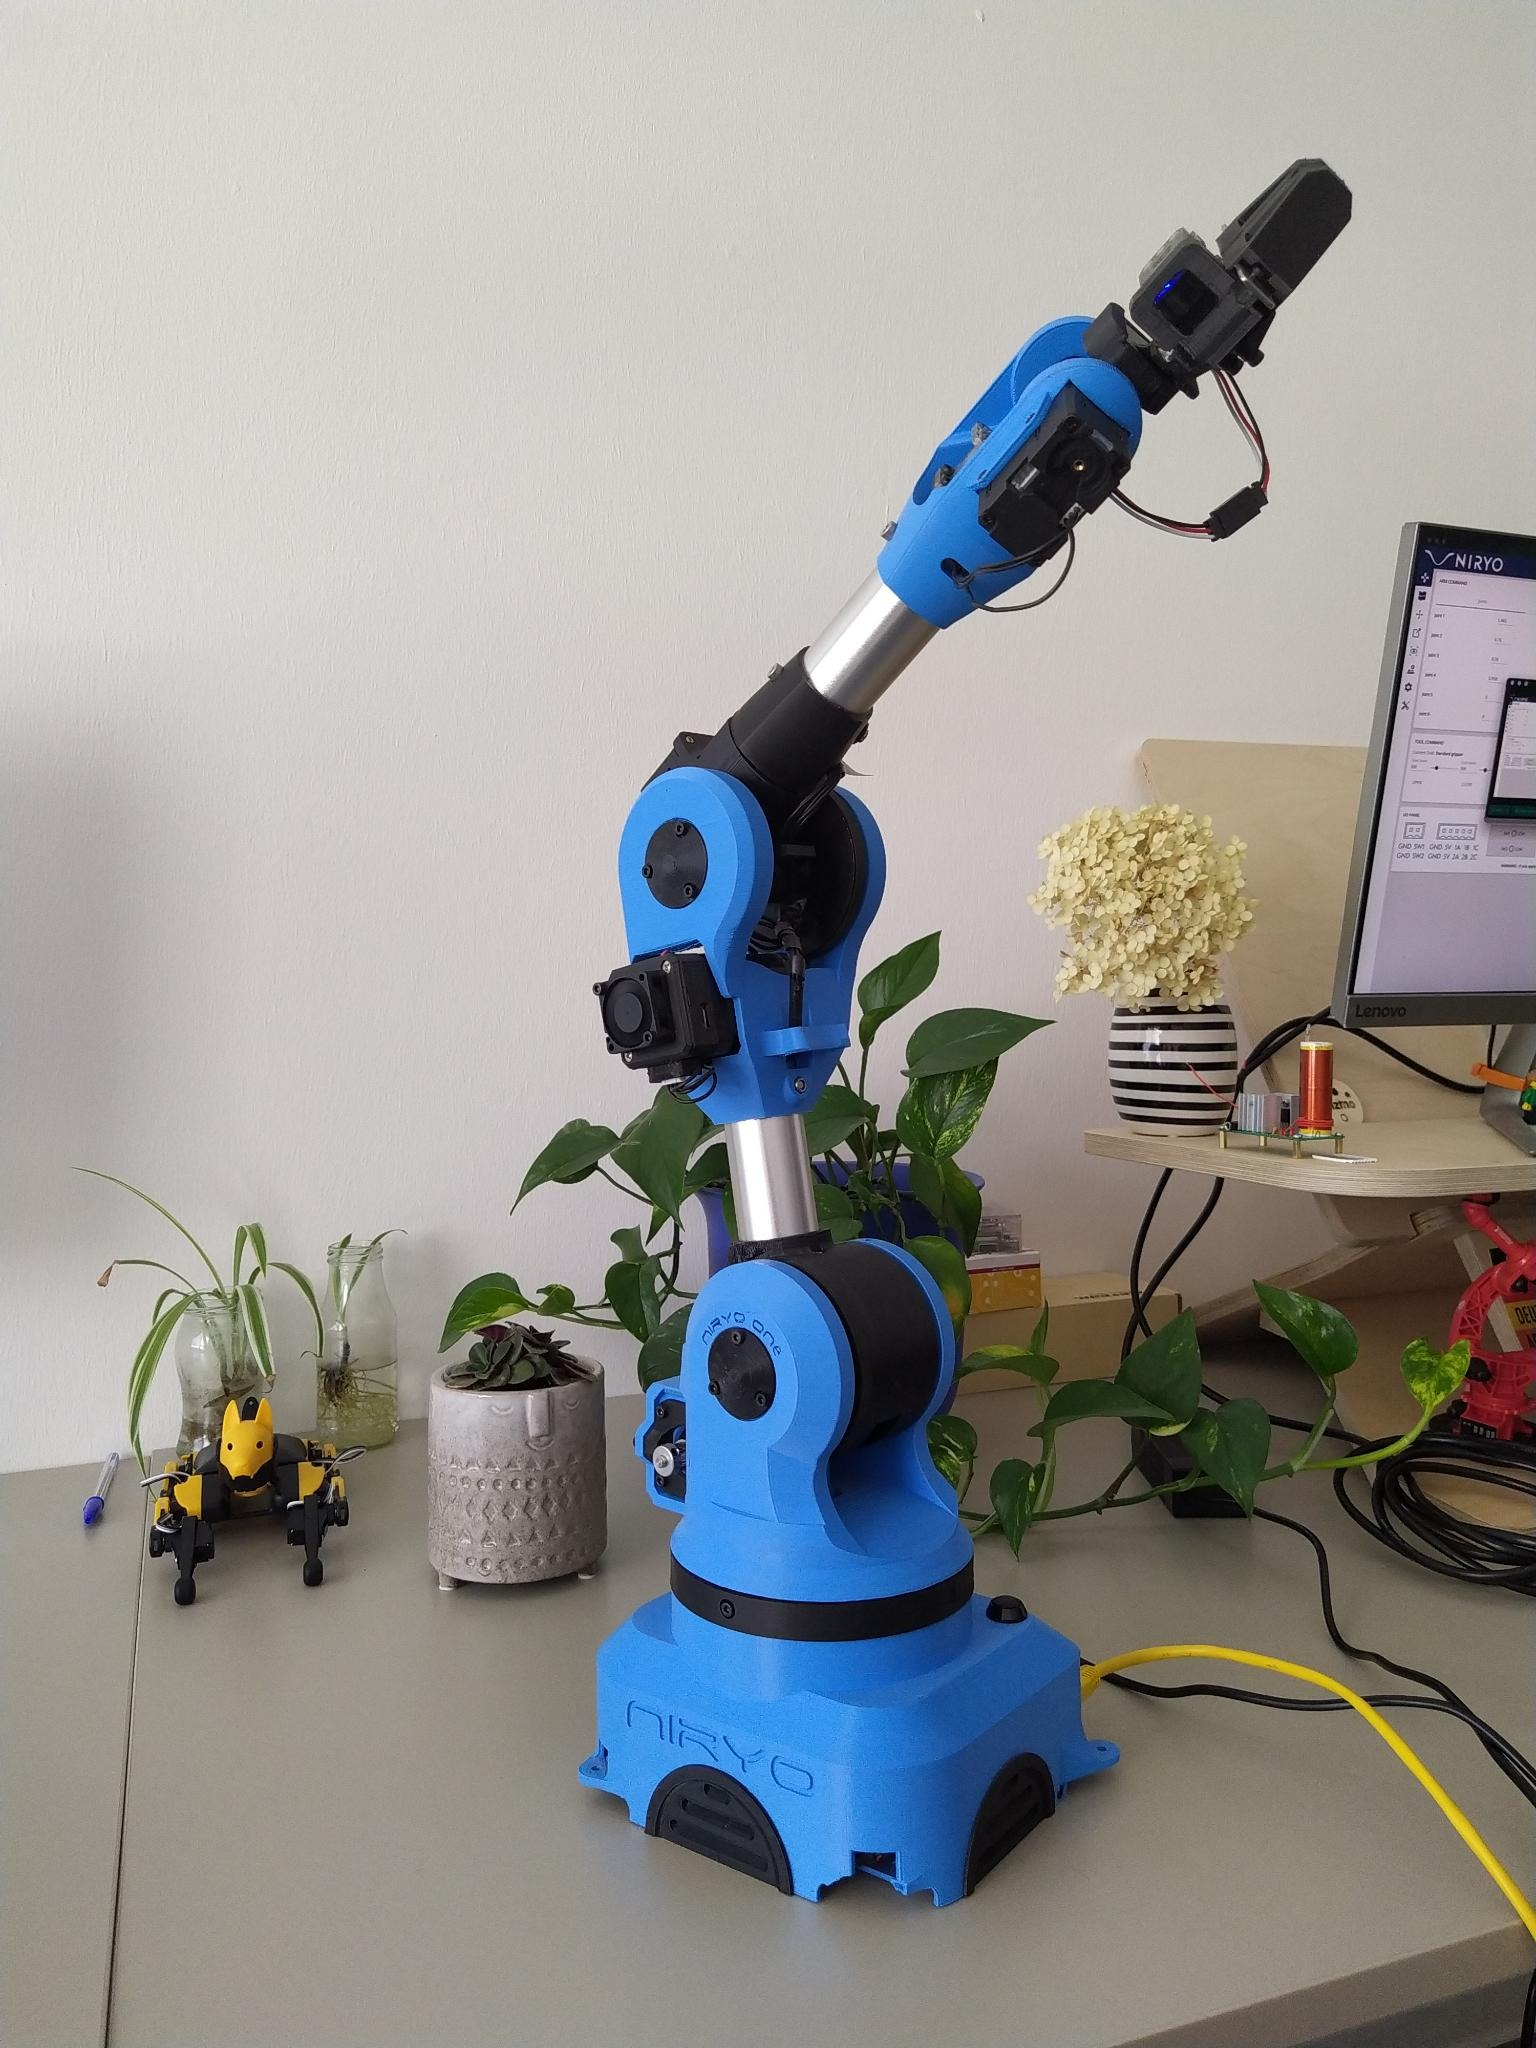
\includegraphics[height=5cm]{Images/07_niryo.jpeg}
            \caption{Niryo One robot}
            \label{fig:niryoRobot}
        \end{subfigure}%
        \begin{subfigure}{.7\textwidth}
            \centering
            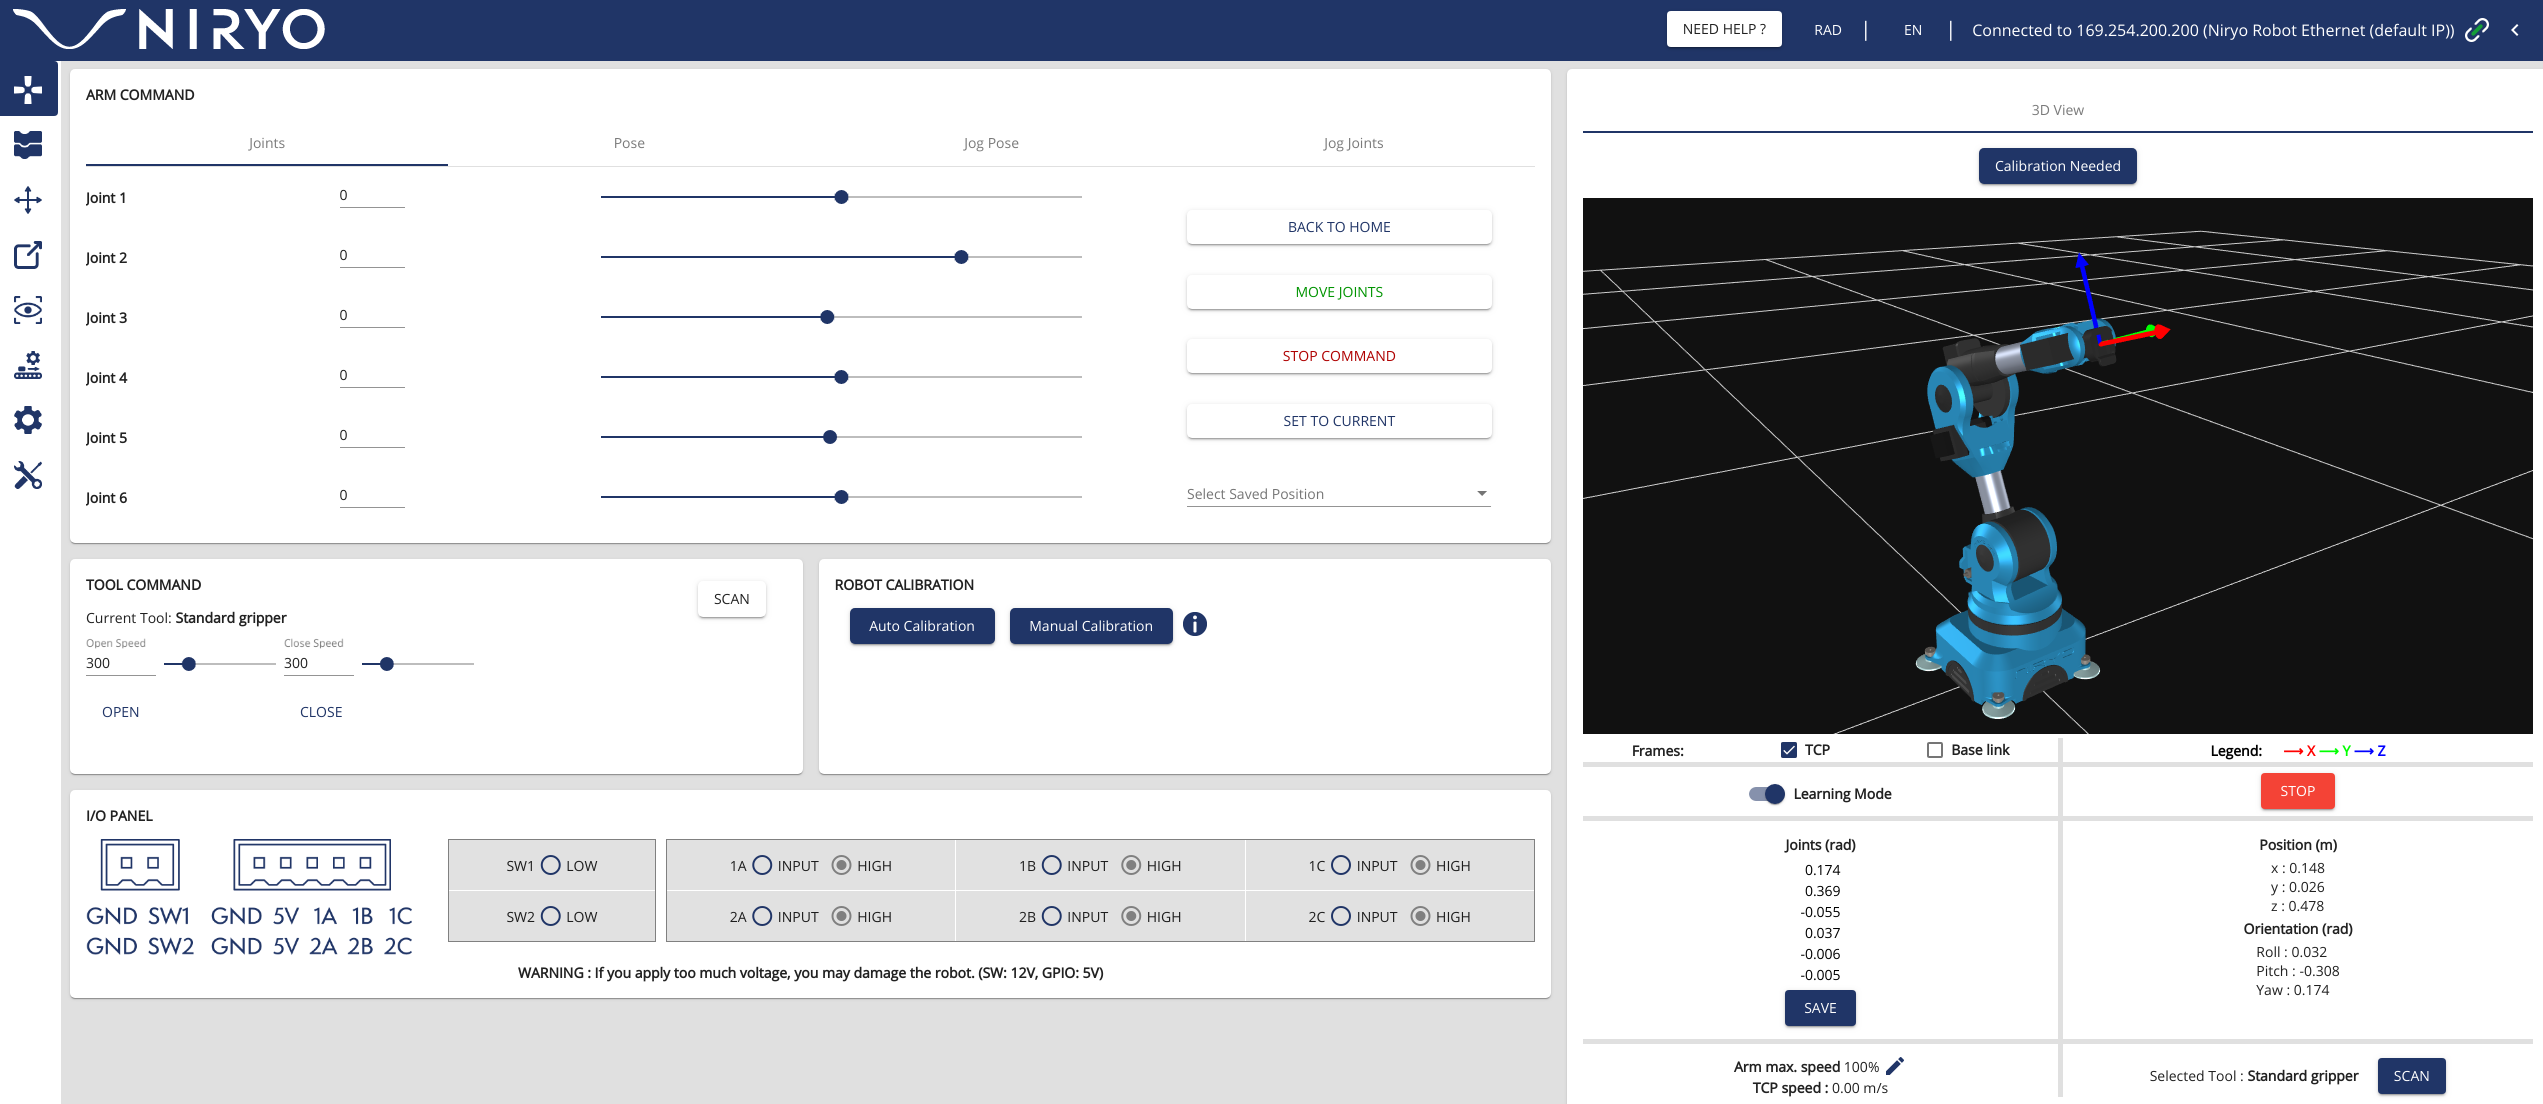
\includegraphics[height=5cm]{Images/07_niryoStudio.png}
            \caption{Niryo Studio}
            \label{fig:niryoStudio}
        \end{subfigure}
        \caption{Calibration of the Niryo robot through an Ethernet connection to the Niryo Studio}
        \label{fig:calibration}
    \end{figure}

\section{Workshops}

    \begin{figure}[h]
        \centering
        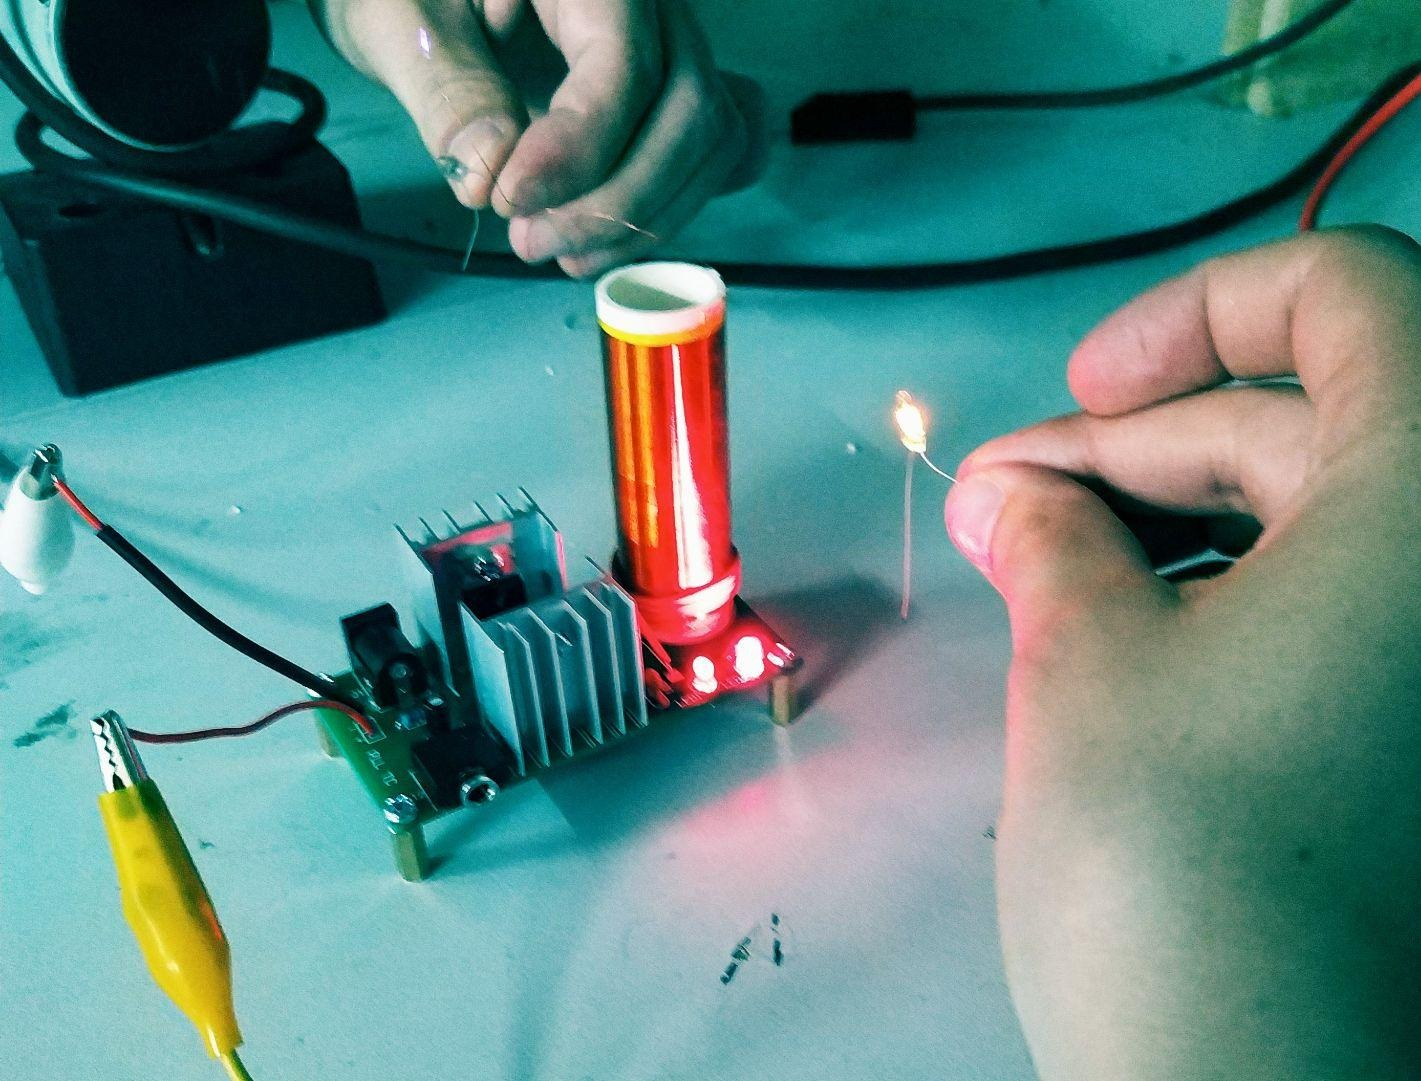
\includegraphics[width=0.5\linewidth]{Images/07_tesla.jpeg}
        \caption{Tesla coil built during the electronics lab workshop}
        \label{fig:tesla}
    \end{figure}

    As part of my extracurricular education, I attended two makerspace workshops this week. The first workshop was related to the use of the electronics laboratory, during which basic skills such as soldering and using electronic measuring systems like multi-meters and oscilloscopes were taught by building a miniature Tesla coil (Figure \ref{fig:tesla}). The second workshop was focused on laser cutting techniques, during this workshop I learned about laser-cutting materials, design, and the best practices for adjusting equipment settings. The skills learned are vital for development of robotic prototypes and to augment the Niryo One and Bittle robots in the laboratory.



\section{Future Work}

    Given the number of issues with the Gazebo extension, its development will continue. It will be necessary to fix the CORB issue to properly display the Gazebo website again. Afterwards, the extension still needs to be tested with a running Gazebo bridge and server. And furthermore, there is plenty of experimentation and testing left to do with Niryo and Bittle.